\documentclass[9pt,twocolumn,twoside]{../../styles/osajnl}
\usepackage{fancyvrb}
\journal{i524} 

\title{OpenStack Nova: Compute Service of OpenStack Cloud}

\author{Kumar Satyam}

\affil[1]{School of Informatics and Computing, Bloomington, IN 47408, U.S.A.}

\affil[*]{Corresponding authors: ksatyam@indiana.edu}

\dates{paper-2, \today}

\ociscodes{Cloud,OpenStack,Nova, API, I524}

% replace this with your url in github/gitlab
\doi{\url{https://github.com/satyamsah/sp17-i524/blob/master/paper2/S17-IR-2031/report.pdf}}


\begin{abstract}
OpenStack Nova is the compute service of the OpenStack cloud system.It is designed to manage and automate the pools of computer resources and can work on bare metal and high performance computing. It is written in python.We will discuss the main components included in the Nova Architecture \cite{www-nova-wiki}.
 
\hfill \break
\end{abstract}

\setboolean{displaycopyright}{true}

\begin{document}

\maketitle


\section{Introduction}
Nova is responsible for spawning vm instances in openstack environment. It is built on a messaging architecture which runs on several servers. This architecture allows components to communicate through a messaging queue. Nova together shares a centralized SQL-based database for smaller deployment. For large deployments an aggregation is used to manage data across multiple data stores\cite{www-nova-official}.

\begin{figure}[htbp]


\section{Architecture -OpenStack Nova}

\hfill \break
\centering
\fbox{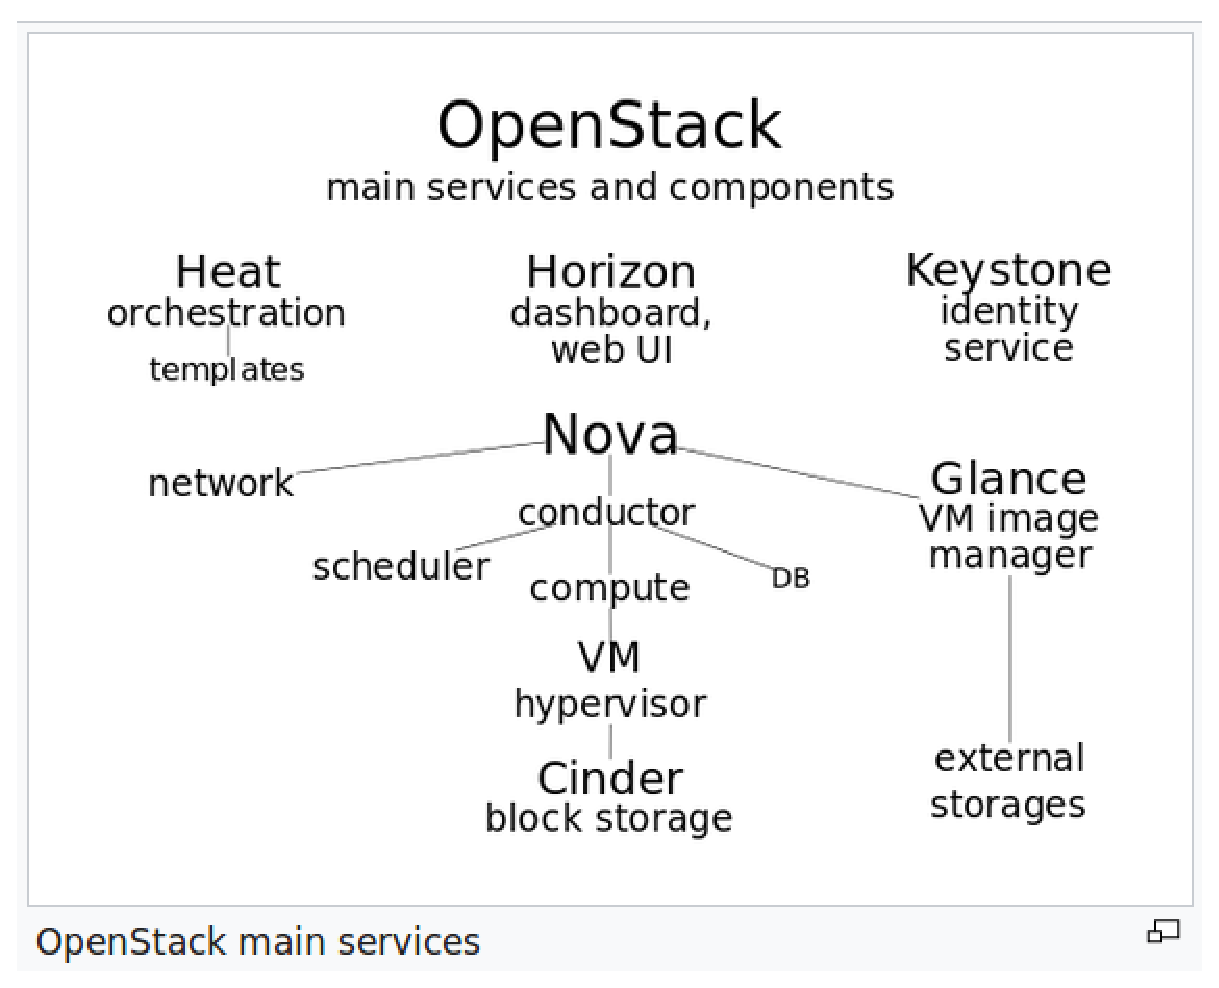
\includegraphics[width=\linewidth]{images/sample}}
\caption{Architecture of OpenStack cloud using Nova \cite{www-nova-pic}  }
\label{fig:false-color}

\end{figure}


\section{Nova Framework}


Nova is comprised of multiple server processes, each performing different functions. The OpenStack provided user interface for Nova which is a REST API. During invocation of the API, the Nova communicates via  RPC (Remote procedure call) passing mechanism.

The API servers process REST requests, which typically involve database reads/writes. RPC messaging is done via the 'oslo.message' library. Most of the nova components can run on different servers and have a manager that is listening for RPC messages. One of the components is Nova Compute where a single process runs on the hypervisor it is managing.

Nova has a centralized database that is logically  shared between all components\cite{www-nova-pepple}.


\section{Nova Components}

Below are the major components of Nova:


\begin{flushleft}


DB: An SQL database for data storage.This is the SQLAlchemy-compatible database. The database name is 'nova'. The 'nova-conductor' service is the only service that writes to the database. 
\end{flushleft}

\begin{flushleft}
\item API: It is the component that receive HTTP requests, converts commands and communicates with other components via the 'oslo.messeging' queue or HTTP.
The 'python-novaclient 7.1.0' is a python binding to OpenStack Nova API which acts as a client for the same. The nova-api provides an endpoint for all API queries (either OpenStack API or EC2 API), initiates most of the orchestration activities (such as running an instance) and also enforces some policy (mostly quota checks)
\end{flushleft}

\begin{flushleft}

Schedular: The 'nova-schedular' is a service to determine how to dispatch compute requests.For example, it determines on which host a VM should launch. Compute is configured with a default scheduler options in the /etc/nova/nova.conf file\cite{www-nova-schedular}.
\end{flushleft}


\begin{flushleft}

Network: It manages IP forwarding, bridges, and vlans. The network controller with nova-network provides virtual networks to enable compute servers to interact with each other and with public network. Compute with nova-network support the following modes, which are implemented as Network Manager types:
\begin{itemize}

\item Flat Network Manager

\item Flat DHCP Network Manager

\item VLAN Network Manger

\end{itemize}

\end{flushleft}


\begin{flushleft}

volume : It manages creation, attaching and detaching of persistent volumes to compute instances. This functionality is being migrated to Cinder, a separate OpenStack service

\end{flushleft}


\begin{flushleft}
Compute: It manages communication with hypervisor and virtual machine

\end{flushleft}


\begin{flushleft}

Conductor: It handles requests that need coordination, acts as a database proxy, or handles object conversions

\end{flushleft}




\section{Step by Step invocation of OpenStack Nova service}

\begin{itemize}

\item Authenticating against the nova-api endpoint

\item Listing instances

\item Retrieving an instance by name and shutting it down

\item Booting an instance and checking status

\item Attaching Floating IP address

\item Changing a security group 

\item Retrieving console login

\end{itemize}

\section{Nova and other Openstack service}

Nova is the main Openstack services as it interact with all the services to set IAAS stack.
Nova interact with Glance service to provided images for VM provisioning.It also interact with the Queue service via a nova-scheduler and nova-conductor API.It interacts with Keystone for authentication and authorization services. It also interacts with Horizon for web interface.

\section{Nova dependence on AMQP}
AMQP is the messaging technology chosen by the OpenStack cloud.The AMQP sits between any two Nova components and allow them to communicate in a loosely coupled fashion. Nova Components use RPC to communicate to one another.It is build on the pub/sub paradigm to have the benefits. Decoupling between client and server(such that the client does not need to know where the servant's reference is) is a major advantage of AMQP\cite{www-nova-amqp}.

\section{Orchestration Task in Nova}
Nova-Conductor service plays an important role to manage the execution of workflows which involve the scheduler. Rebuild, resize, and building the instance are managed here. This was done in order to have better separation of responsibilities between what compute nodes should handle and what schedular should handle and to clean up the path of execution. In order to query the schedular in a synchronous manner it needed to happen after the API had returned a response otherwise API response times would increase and thats why conductor was chosen. And changing the schedular call from asynchronous to synchronous helped to clean up the code\cite{www-nova-orchestrator}.

The earlier logic was complicated and the scheduling logic was distributed across the code.The earlier process was changed to the following:

\begin{itemize}
\item API receives request to build an instance.
\item API sends an RPC cast to conductor to build an instance.
\item Conductor sends an RPC call to schedular to pick a compute and waits for the response. If there is a schedular fail, it stops the build at the conductor.
\item Conductor sends an RPC cast to the compute to build the instance. If the build succeeds, stop here. If it fails then the compute sends an RPC cast to conductor to build an instance. This is the same RPC message that was sent by the API.

\end{itemize}



\section{OpenStack Nova Support}
Earlier Openstack was supported on KVM but its support has been extended QEMU. Microsoft Hyper -V and Vmware ESXi too provide extended support. Nova has support for XenServer and XCP through XenAPI virtual layer.It also support bare metal deployment and provisioning from 'Ironic' version. This means it is possible to deploy virtual machines. By default, it will use PXE and IPMI to provision and turn on/off the machine. But from the Ironic version it support vendor-specific plugins which may implement additional functionality. 


\section{OpenStack Nova in Bigdata}

A use case has been developed to leverage OpenStack to perform big data analytics. OpenStack used cassandra database for columnar data structure. PostgreSQL for relational data structure.This use case also allows us to configure Hadoop distributed file system for large unstructured data. OpenStack Sahara has come up with core cloud components of Big data\cite{www-nova-bigdata}.

\section{OpenStack Nova and other competitors}
 The OpenStack nova does the same task as it is being done by AWS EC2, Google CE and Microsoft Azure VM. With respect to Beach marking the main difference is the cloud administrator can upload their images in OpenStack where as in AWS and Google Cloud storage, one need to use the pre-defined list.The AWS is used mainly as public cloud where as the Openstack can be used a private cloud. But OpenStack has an advantage of customizing our own cloud configuration which is not there in any of the vendor specific clouds.

\section{conclusion}

We discussed about the main components of OpenStack Nova and how it is interacting with different other Openstack services.We also showed use case of running big data problem on Openstack. We also discussed the compute service offerings provided by cloud vendors other than OpenStack.

\bibliography{references}

\end{document}
